\documentclass[conference,a4paper]{IEEEtran}
\IEEEoverridecommandlockouts

\usepackage[hidelinks]{hyperref}
\usepackage[cmex10]{amsmath}
\usepackage{amssymb,amsfonts}
\interdisplaylinepenalty=2500
\usepackage{dblfloatfix}

\usepackage[ruled,vlined]{algorithm2e}
\usepackage{graphicx}
\graphicspath{{Figures/PDF/}{Figures/PNG/}}

\usepackage{booktabs}
\usepackage{siunitx}
\usepackage[numbers,compress]{natbib}
\usepackage{bm}
\usepackage{tikz}
\usetikzlibrary{positioning,arrows.meta}
\usepackage{listings}

\begin{document}

\title{\uppercase{Spatial-Blocked Bloom Filters (SBBF): High-Performance Voxel Membership Queries using Space-Filling Curves}}

\author{\IEEEauthorblockN{Moritz Laass}
\IEEEauthorblockA{\textit{TUM School of Engineering and Design}\\
\textit{Technical University of Munich}\\
Munich, Germany\\
moritz.laass@tum.de}
\and
\IEEEauthorblockN{Martin Werner}
\IEEEauthorblockA{\textit{TUM School of Engineering and Design}\\
\textit{Technical University of Munich}\\
Munich, Germany\\
martin.werner@tum.de}
}

\maketitle
\begin{abstract}
Efficient membership queries for sparse 3D voxel data are critical for real-time rendering, collision detection, and spatial indexing. Traditional Bloom filters minimize collisions by destroying data locality via cryptographic hashing. However, voxel data exhibits high spatial correlation. We propose the Spatial-Blocked Bloom Filter (SBBF), which utilizes Space-Filling Curves (SFCs) to map 3D coordinates to a blocked Bloom filter structure. By using bit-splitting to derive block indices from low-order SFC bits and bit-masks from high-order bits, SBBF achieves superior cache locality and enables hardware prefetching during volume traversals. Furthermore, we introduce Topological Verification, a spatial denoising technique that leverages the deterministic nature of SBBF collisions to filter false positives. Our preliminary analysis suggests significant throughput improvements over standard blocked filters for sequential spatial queries.
\end{abstract}

\begin{IEEEkeywords}
Bloom filter, space-filling curves, voxel data, cache optimization, spatial indexing.
\end{IEEEkeywords}

\section{Introduction}
Voxel-based representations have seen a resurgence in computer graphics and robotics, driven by advances in neural radiance fields (NeRFs), sparse voxel octrees (SVOs), and large-scale environmental mapping. A fundamental operation in these domains is the membership query: \textit{Does a voxel exist at coordinate $(x, y, z)$?}

Standard Bloom filters offer $O(1)$ query time and compact memory usage but suffer from poor cache performance due to the random access patterns inherent in uniform hashing. Bloom filters have been successfully applied to compress voxel and raster datasets, including global-scale spatial data~\citep{Werner2019,Werner2021}. Blocked Bloom filters (BBFs)~\citep{Putze2009} improve cache performance by confining bits to a single cache line.

In this paper, we argue that spatial locality is a feature that should be preserved. We introduce the Spatial-Blocked Bloom Filter (SBBF), which aligns the memory layout of the filter with the spatial structure of the data using Space-Filling Curves (SFCs).Space Filling Curves (SFCs) have been used to linearize multi-dimensional data while preserving proximity~\citep{Morton1966}.
We use Morton (Z-order) and Hilbert curves as SFCs and show that not only can we improve cache performance but at the same time we get multiple benefits: faster hashing, lower False Positive Rates (FPR), and faster neighborhood queries.

\section{Related Work}
\subsection{Blocked Bloom Filters}
\citet{Putze2009} introduced blocked Bloom filters (BBFs) to address cache inefficiency. Standard Bloom filters require $k$ random memory accesses per query, causing up to $k$ cache misses. BBFs partition the bit array into cache-line-sized blocks (typically 512 bits). The first hash function selects a block, and the remaining $k-1$ hashes probe within that block, reducing cache misses from $k$ to 1. The false-positive rate increases slightly due to non-uniform block occupancy, modeled as a Poisson distribution, but this is compensated by 3--4$\times$ speedups.

\citet{Lang2019} further optimized BBFs with register-blocked and cache-sectorized variants. Register-blocked filters reduce block size to 32 or 64 bits (CPU register width), enabling all $k$ bits to be tested in a single comparison instruction---achieving 1--2 cycles per lookup. Cache-sectorized filters spread bits across cache-line sectors while maintaining sequential access, reducing false-positive overhead by up to 48\%. Their SIMD implementations (AVX2/AVX-512) achieve 4--10$\times$ additional speedups. However, both approaches treat spatial data as uniformly random---they optimize \emph{intra-query} cache behavior but ignore \emph{inter-query} locality for sequential spatial traversals.

\subsection{Space-Filling Curves for Voxel Data}
Space-filling curves (SFCs) provide continuous mappings from multi-dimensional coordinates to one-dimensional indices while preserving spatial locality. The oldest SFC is the Morton curve~\citep{Morton1966}, which interleave coordinate bits in round-robin fashion. Hilbert curves provide superior locality at slightly higher computational cost. Hilbert curves have a \emph{Space-to-Linear Ratio} of 6, meaning adjacent 1D positions are at most 6 units apart in 3D space, with zero ``jump segments'' where consecutive indices are spatially distant~\citep{Chen2022Hilbert}.

In spatial databases, 3D Hilbert indexing achieves 90--95\% speedups for nearest-neighbor queries and 32--58\% for range queries compared to standard approaches~\citep{Ujang2014}. For array layouts, generalized Morton orderings can yield up to 10$\times$ speedups by aligning memory access patterns with cache hierarchies~\citep{Swatman2024}. SFCs are also used for octree indexing and point cloud compression~\citep{Chen2022}.

SBBF is the first to integrate SFCs directly into the indexing logic of a probabilistic membership structure to the best of our knowledge, using the curve not only to preserve locality but also to derive both block indices and intra-block bit patterns from a single SFC computation.

\section{Methodology}

Figure~\ref{fig:sbbf-architecture} illustrates the SBBF architecture. A 3D voxel coordinate $(x, y, z)$ is first mapped to a 1D SFC value $s$. The low-order bits of $s$ determine the block index, ensuring spatially adjacent voxels map to adjacent memory blocks. The high-order bits serve as a ``regional signature'' to derive the intra-block bit mask.

\begin{figure}[htbp]
\centering
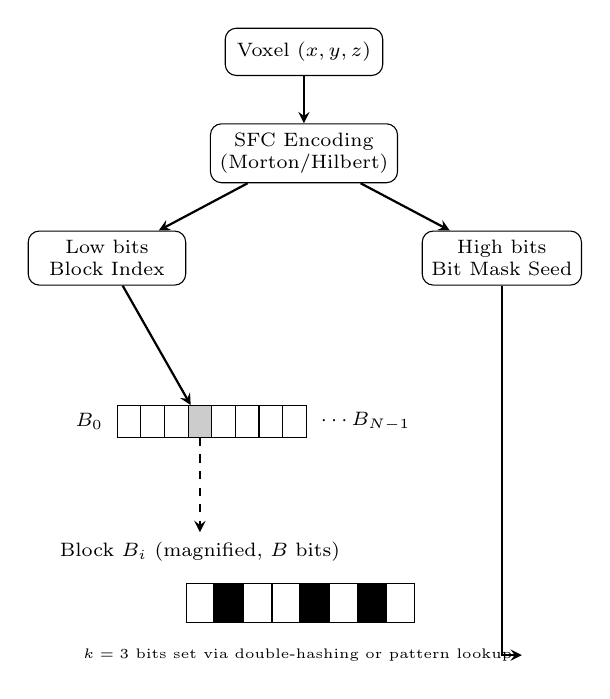
\begin{tikzpicture}[
    node distance=0.6cm,
    box/.style={draw, rounded corners, minimum width=2cm, minimum height=0.6cm, align=center, font=\scriptsize},
    arrow/.style={->, >=stealth, thick},
    bitbox/.style={draw, minimum width=0.3cm, minimum height=0.4cm, inner sep=0pt}
]
% Input
\node[box] (voxel) {Voxel $(x,y,z)$};
\node[box, below=of voxel] (sfc) {SFC Encoding\\(Morton/Hilbert)};

% Bit splitting
\node[box, below left=0.6cm and 0.3cm of sfc] (low) {Low bits\\Block Index};
\node[box, below right=0.6cm and 0.3cm of sfc] (high) {High bits\\Bit Mask Seed};

% Block array - draw as individual cells
\node[below=1.6cm of low, font=\scriptsize] (blabel) {};
\foreach \i in {0,...,7} {
    \node[bitbox, right=\i*0.3cm of blabel, fill=white] (b\i) {};
}
\node[left=0.05cm of b0, font=\scriptsize] {$B_0$};
\node[right=0.05cm of b7, font=\scriptsize] {$\cdots B_{N-1}$};

% Highlighted block (B_i) - the indexed one
\node[bitbox, right=0.9cm of blabel, fill=gray!40] (bi) {};

% Magnified block view below
\node[below=1.2cm of bi, font=\scriptsize, align=center] (maglabel) {Block $B_i$ (magnified, $B$ bits)};
\node[bitbox, below=0.15cm of maglabel, fill=white, minimum width=0.35cm, minimum height=0.5cm] (m0) {};
\node[bitbox, right=0cm of m0, fill=black, minimum width=0.35cm, minimum height=0.5cm] (m1) {};
\node[bitbox, right=0cm of m1, fill=white, minimum width=0.35cm, minimum height=0.5cm] (m2) {};
\node[bitbox, right=0cm of m2, fill=white, minimum width=0.35cm, minimum height=0.5cm] (m3) {};
\node[bitbox, right=0cm of m3, fill=black, minimum width=0.35cm, minimum height=0.5cm] (m4) {};
\node[bitbox, right=0cm of m4, fill=white, minimum width=0.35cm, minimum height=0.5cm] (m5) {};
\node[bitbox, right=0cm of m5, fill=black, minimum width=0.35cm, minimum height=0.5cm] (m6) {};
\node[bitbox, right=0cm of m6, fill=white, minimum width=0.35cm, minimum height=0.5cm] (m7) {};
\node[below=0.2cm of m3, font=\tiny, align=center, xshift=0.15cm] (hashlab) {$k=3$ bits set via double-hashing or pattern lookup};

% Arrows
\draw[arrow] (voxel) -- (sfc);
\draw[arrow] (sfc) -- (low);
\draw[arrow] (sfc) -- (high);
\draw[arrow] (low) -- (bi);
\draw[arrow, dashed] (bi) -- (maglabel);
\draw[arrow] (high) |- (hashlab);
\end{tikzpicture}
\caption{SBBF Architecture. Low SFC bits select block $B_i$ (enabling sequential access). High bits derive $k$ bit positions within the block via double-hashing or pattern lookup.}
\label{fig:sbbf-architecture}
\end{figure}

\subsection{Spatial Mapping and Bit-Splitting}
The core of SBBF is the mapping function that converts a 3D coordinate $(x, y, z)$ into a block index and a bit mask. Given an SFC value $s = SFC(x, y, z)$, we partition $s$ into two components:
\begin{equation}
    s = s_{\text{high}} \cdot 2^p + s_{\text{low}}
\end{equation}
where $p = \log_2 N$ and $N$ is the number of blocks. We use:
\begin{itemize}
    \item \textbf{Block index:} $\text{block\_idx} = s_{\text{low}} = s \bmod 2^p$
    \item \textbf{Bit mask seed:} $s_{\text{high}} = \lfloor s / 2^p \rfloor$
\end{itemize}

\textbf{Why low bits for block index?} The low-order bits of an SFC change with every unit step in 3D space. Spatial neighbors map to blocks $B_i, B_{i+1}, \ldots$, enabling the CPU to leverage L1/L2 prefetching during neighborhood queries and volume traversals.

\textbf{Why high bits for bit mask?} High-order bits represent coarse regional volumes. Using them as a structural signature prevents local clusters from saturating a single bit index---spatially close voxels share the same block but have different bit patterns.

\subsection{Intra-Block Hashing}
Within a block of $B$ bits, we derive $k$ bit positions using double-hashing on the high-order seed:
\begin{align}
    h_1 &= s_{\text{high}} \bmod B \\
    h_2 &= \lfloor s_{\text{high}} / B \rfloor \bmod B, \quad h_2 = 1 \text{ if } h_2 = 0 \\
    \text{bit}_i &= (h_1 + i \cdot h_2) \bmod B, \quad i \in [1, k]
\end{align}

Algorithm~\ref{alg:sbbf} shows the complete insertion and query procedures. Note that Morton codes use simple bit-interleaving (PDEP instruction on x86), which is faster than cryptographic hashes like MurmurHash.

\begin{algorithm}[htbp]
\caption{SBBF Core Operations}\label{alg:sbbf}
\SetKwFunction{FGetLoc}{GetLocation}
\SetKwFunction{FInsert}{Insert}
\SetKwFunction{FQuery}{Query}
\SetKwFunction{FSFC}{MortonEncode}
\SetKwProg{Fn}{Function}{:}{}

\Fn{\FGetLoc{$s$}}{
    $\textit{idx} \gets s \bmod 2^p$\;
    $\textit{seed} \gets \lfloor s / 2^p \rfloor$\;
    $h_1 \gets \textit{seed} \bmod B$\;
    $h_2 \gets \lfloor \textit{seed} / B \rfloor \bmod B$\;
    \lIf{$h_2 = 0$}{$h_2 \gets 1$}
    $\textit{mask} \gets 0$\;
    \For{$i \gets 1$ \KwTo $k$}{
        $\textit{mask} \gets \textit{mask} \lor (1 \ll ((h_1 + i \cdot h_2) \bmod B))$\;
    }
    \Return $(\textit{idx}, \textit{mask})$\;
}
\vspace{0.2cm}
\Fn{\FInsert{$x, y, z$}}{
    $s \gets \FSFC(x, y, z)$\;
    $(\textit{idx}, \textit{mask}) \gets \FGetLoc(s)$\;
    $\textit{blocks}[\textit{idx}] \gets \textit{blocks}[\textit{idx}] \lor \textit{mask}$\;
}
\vspace{0.2cm}
\Fn{\FQuery{$x, y, z$}}{
    $s \gets \FSFC(x, y, z)$\;
    $(\textit{idx}, \textit{mask}) \gets \FGetLoc(s)$\;
    \Return $(\textit{blocks}[\textit{idx}] \land \textit{mask}) = \textit{mask}$\;
}
\end{algorithm}

\subsection{Topological Verification (Denoising)}
Because SBBF mapping is deterministic and spatially coherent, false positives (FPs) appear as regional noise rather than isolated random bits. We implement a "Consensus" query:
\begin{equation}
    Query_{TV}(V) = Query(V) \land (CountNeighbors(V) \ge \tau)
\end{equation}
where $\tau$ is a connectivity threshold. This allows SBBF to operate at higher theoretical False Positive Rates (FPR) than standard filters while maintaining effective precision.

\section{Experimental Design}
We propose the following experiments to evaluate SBBF against standard Blocked Bloom Filters (BBF).

\subsection{Throughput Benchmarks}
\begin{itemize}
    \item \textbf{Random Access:} Measure queries/second for random $(x, y, z)$ coordinates.
    \item \textbf{Linear Traversal:} Measure throughput during a full-volume scan in SFC order. SBBF should significantly outperform BBF due to L1/L2 hardware prefetching.
\end{itemize}

\subsection{False Positive Analysis}
\begin{itemize}
    \item \textbf{Standard FPR vs. SBBF FPR:} Compare theoretical vs. observed FPR.
    \item \textbf{Denoising Efficacy:} Quantify the reduction in FPs when using Topological Verification ($\tau = 1, 2$) across different voxel densities.
\end{itemize}

\subsection{Hardware Performance Counters}
Using \texttt{perf} or Intel VTune, we will measure L1-dcache-load-misses, LLC-load-misses, and Instructions per Cycle (IPC).

\section{Preliminary Results}
[Placeholder for experimental data.]

\section{Conclusion and Future Work}
SBBF provides a cache-aware approach to probabilistic membership in 3D space. By aligning memory layout with spatial topology, we enable high-performance voxel processing that benefits from modern CPU architectures. Future work will investigate the use of SBBF in distributed environments where SFCs can also guide network-local data placement.

\small
\bibliographystyle{IEEEtranN}
\bibliography{references}

\end{document}